\subsection{\acs{NEF}}
\label{chap:impl:exposure:nef}

As it has been repeatedly noted throughout this document, the \acs{NEF} is the primary network function of the \acs{5GC} \acs{SBA} responsible for the exposure of network capabilities to third parties. The testbed developed in this work follows the same principle, relying on the \acs{NEF} as the primary entry point for external interactions with the \acs{5GC}.

Based on the analysis of the available \acs{NEF} implementations conducted in Section~\ref{exposure:NEFimplementations}, the NEFSim~\cite{NEFsim}, as extended by \acs{ITAv}~\cite{NEFemulatorAtnog}, was selected as the most suitable choice for this role within the testbed. This selection was motivated by a variety of factors:

\begin{enumerate}
    \item \textbf{Wider coverage of \acs{NEF} northbound \acs{API} suite}~\cite{ETSI_TS_129_522_V18_11_0}\textbf{:} including the \textit{PfdManagement}, \textit{MonitoringEvent}, \textit{AsSessionWithQoS} and \textit{TrafficInfluence} \acsp{API} \fix{COMPLETE THIS};
    \item \textbf{Built-in Integration with \acs{CAPIF}:} among the analyzed implementations, it is the only one which supports, or even considers, authentication, authorization and service discovery capabilities, using the \acs{CAPIF} framework;
    \item \textbf{Simulated Environment:} the NEFSim exposes the standardized set of \acs{NEF} northbound \acsp{API}, allowing network application developers to develop and validate network applications, without requiring access to a fully featured \acs{NEF} instance;
\end{enumerate}

Hence, in its original purpose, the NEFSim establishes a simulated environment which exposes the set of \acs{NEF} northbound \acsp{API}, without depending on an underlying \acs{5G} core deployment. This way, in the original design, all responses produced by the \acsp{API} would be completely decoupled from actual network state, essentially operating as stubs that conform to the specification. This approach is not suitable for a real testbed, where customers expect the opportunity to develop and validate network application behavior against live traffic, with real \acsp{UE} and live \acs{QoS} sessions. Use cases that depend on network conditions observed during execution, such as throughput and latency, cannot be verified through simply simulated responses.

Therefore, at \acs{ITAv}, there is an ongoing effort to integrate the \acs{NEF}Sim implementation with the \acs{5G} network, extending its role beyond a purely simulated environment and allowing application developers to actually incorporate network behavior into their business logic. This is the case for the \textit{AsSessionWithQoS} \acs{API}, but does not yet cover most of the supported northbound \acsp{API} described previously.

Thus, in the scope of this dissertation, the \acs{NEF}Sim implementation is extended along two distinct dimensions. First, the \textit{AsSessionWithQoS} \acs{API} was partially reimplemented to integrate with an updated version of the \acs{ITAv} Slice Manager, already used on the generic controller implementation, which interacts with the Huawei \acs{5G} network to control session \acs{QoS} within a given slice. Second, the \textit{AnalyticsExposure} \acs{API} was developed from scratch and integrated with the testbed's observability mechanisms, to expose real network metrics to external consumers. By combining these two \acsp{API}, network application developers are equipped with the instruments to both influence and observe network behavior according to their application requirements: configuring and enforcing specific \acs{QoS} requirements through the \textit{AsSessionWithQoS} \acs{API}, while monitoring and reacting to live network conditions, with the \textit{AnalyticsExposure} \acs{API}.

\subsubsection{AsSessionWithQoS \acs{API}}
\label{chap:impl:exposure:nef:AsSessionWithQoS}

The \textit{AsSessionWithQoS} \acs{API}, defined in \acs{3GPP} TS~29.522~\cite{ETSI_TS_129_522_V18_11_0}, allows an \acs{AF} to request a specific \acs{QoS} for the traffic of a given \acs{UE}, by creating a subscription resource at the \acs{NEF}. Each subscription identifies the target \acs{UE}, the requested \acs{QoS}, and a notification destination to which the \acs{NEF} reports relevant events throughout the session's lifetime (e.g. failed resources allocation). In the \acs{ITAv}'s \acs{NEF}Sim current implementation~\cite{NEFemulatorAtnog}, the endpoints of this \acs{API} are decoupled from the network through a driver interface, which exposes two operations: changing the \acs{QoS} of a set of \acsp{UE}, and reverting it to its default values. Two drivers implement this interface, a no-operation driver, which preserves the original simulated behavior, and a Huawei driver, which applies the requested \acs{QoS} to the \acs{5G} network through the Slice Manager \acs{API}. The active driver is selected at deployment time, through the NEFSim configuration.

The original Huawei driver targeted a previous version of the Slice Manager \acs{API}. The two versions differ substantially with different endpoint definitions and request and response schemas. Furthermore, the previous version processed requests synchronously, whereas the the current version adopts an asynchronous processing model in which each operation is assigned a unique identifier that must be used to subsequently retrieve the execution outcome. The \acs{API} and the driver was therefore adapted to accommodate these changes and ensure compatibility with the current \acs{API} specification. Figure~\ref{fig:impl:exposure:nef:AsSessionWithQoS:sequence} illustrates the interaction sequence between a subscriber, the \acs{NEF} (using the updated driver) and the Slice Manager, highlighting the asynchronous processing for the creation of a \acs{QoS} subscription.

\begin{figure}[htbp]
    \centering
    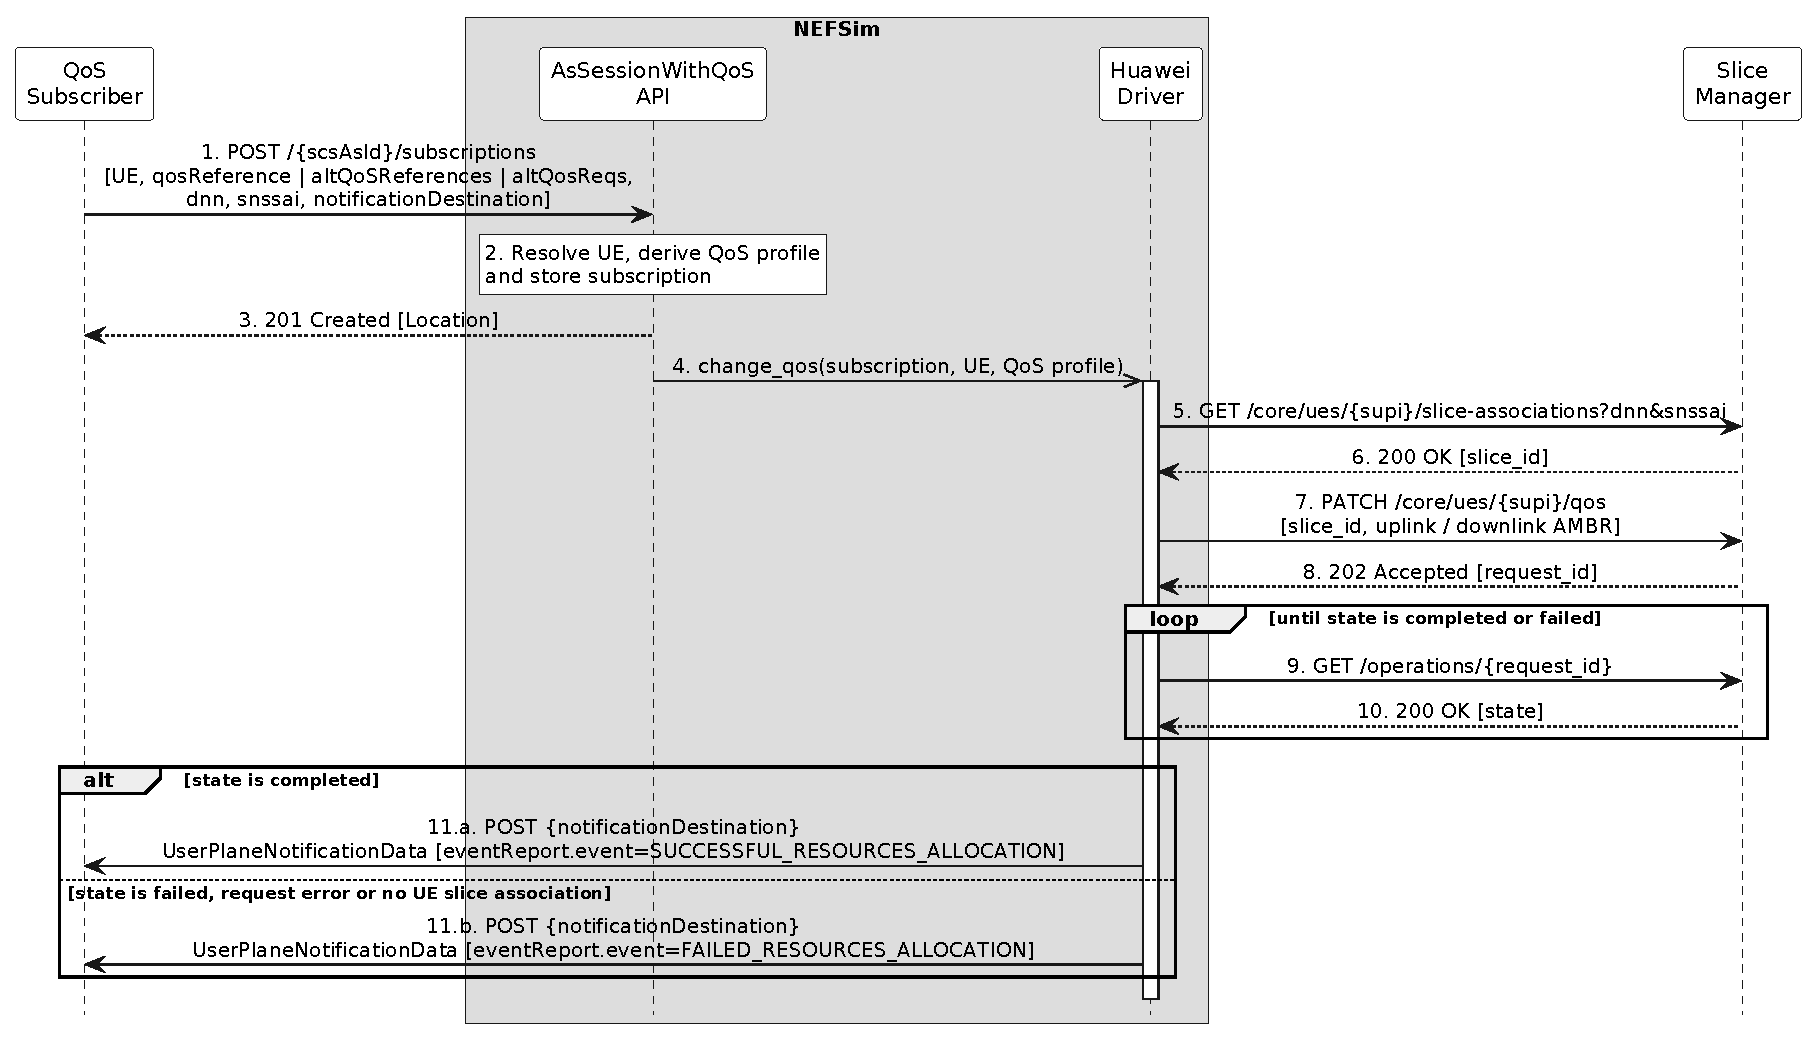
\includegraphics[width=1\linewidth]{figs/plantuml/as-session-with-qos-sequence.pdf}
    \caption{Sequence Diagram for the creation of a \acs{QoS} Subscription via the \textit{AsSessionWithQoS} \acs{API}}
    \label{fig:impl:exposure:nef:AsSessionWithQoS:sequence}
\end{figure}

The \acs{NEF}Sim \textit{AsSessionWithQoS} \acs{API} follows an optimistic, asynchronous model: the \acs{QoS} subscription is acknowledged as successfully created before the requested \acs{QoS} is actually enforced in the network (in this case, the network slice), and the subscriber is only informed of the final outcome later, through a notification.

Upon receiving a subscription request, the \acs{NEF} resolves the target \acs{UE}, derives the \acs{QoS} profile to be enforced, stores the subscription and immediately returns the reference to the subscription resource (steps 1 to 3). The \acs{QoS} profile is extracted from the subscription, either from a QoS reference (\texttt{qosReference} or \texttt{altQoSReferences}), mapped onto a set of preconfigured \acs{QoS} profiles (locally on the \acs{NEF}Sim), or from explicit \acs{QoS} requirements (\texttt{altQosReqs}), such as the uplink and downlink bit rates. The \acs{QoS} enforcement is then delegated to the Huawei driver as a background task (step 4).

Previously, subscriptions containing the \acs{DNN} and \acs{S-NSSAI} attributes were rejected by \acs{NEF}Sim. In the new implementation, these attributes are used to retrieve the slice association of the target \acs{UE} (step 5 and 6). When the subscription does not specify a \acs{DNN}, the one associated with the \acs{UE} in \acs{NEF}Sim is used instead. Once the slice association is retrieved, the driver requests the Slice Manager to update the uplink and downlink aggregate maximum bit rates of the corresponding \acs{UE}-slice association (steps 7). This way, only the \acs{QoS} of the target \acs{UE} is modified, leaving the network slice configuration untouched and ensuring that the remaining \acsp{UE} associated with the slice continue to operate under the default \acs{QoS}. Only the bitrate parameters of the \acs{QoS} profile are mapped to the Slice Manager request, as these are what's supported by the Slice Manager endpoint. If the \acs{UE} is not associated with any network slice matching the subscription, the request fails. The creation of a new network slice by the \acs{NEF} was deliberately left unsupported, since the lifecycle of network slices in the testbed, including the attachment of an \acs{UE} to a newly created slice, is managed by \acs{OSL} and the generic controller, as described in Section~\ref{chap:impl:resource_lifecycle}.

The Slice Manager accepts the request and returns an operation identifier (step 8), which the driver periodically polls until the operation state is reported as either completed or failed (steps 9 and 10). Although this approach enables asynchronous operation tracking, it is not the most efficient solution, as it requires the driver to issue repeated requests to retrieve the operation status. Ideally, this mechanism would be replaced by a callback endpoint, a common approach already adopted by multiple \acs{3GPP} and CAMARA \acsp{API}, allowing the Slice Manager to notify the driver upon completion or failure. However, since callback endpoints are not supported by the Slice Manager, periodic polling remains necessary. Finally, the \acs{NEF} notifies the subscriber with a \texttt{SUCCESSFUL\_RESOURCES\_ALLOCATION} event if the operation was completed, or a \texttt{FAILED\_RESOURCES\_ALLOCATION} event if the operation failed or no matching slice association was found (step 11).

The update and deletion of \acs{QoS} subscriptions follow a similar approach. Depending on the requested \acs{QoS} profile, these operations may trigger a revert operation to restore the \acs{UE} to the default \acs{QoS} configuration of the network slice, similarly requiring the retrieval of the \acs{UE}-slice association from the Slice Manager. As fallback, the \acs{QoS} is instead reverted to the default profile configured in \acs{NEF}Sim.

Under the CAMARA initiative, the same capability is exposed through the more user-friendly \acs{QoD} \acs{API}, which abstracts the underlying \textit{AsSessionWithQoS} procedure from network application developers. Due to this abstraction, no changes were needed to be made to the CAMARA \acs{QoD} \acs{API} already implemented at \acs{ITAv}.

\subsubsection{AnalyticsExposure \acs{API}}
\label{chap:impl:exposure:nef:AnalyticsExposure}

The \textit{AnalyticsExposure} \acs{API}, defined in \acs{3GPP}~TS~29.522~\cite{ETSI_TS_129_522_V18_11_0}, allows external consumers to retrieve analytics information generated by the \acs{5G} System, typically provided by an \acs{NWDAF}. Analytics can be obtained either through fetch requests, answered synchronously with the requested analytics data, or through a subscription-based model where the \acs{AF} can subscribe to network analytics and receive notifications periodically or when specific network conditions are met (e.g. crossing a defined threshold). In the original \acs{NEF}Sim implementation, support was limited to fetch requests for the \texttt{UE\_MOBILITY} event, which returned the simulated position of the target \acs{UE}. However, this implementation did not provide any analytics based on actual network metrics, nor did it offer analytics subscriptions, limiting its ability to expose meaningful insights into network performance and usage for network applications. In addition, since no \acs{NWDAF} is available in the 5GAIner infrastructure, there was no dedicated component from which analytics could be retrieved.

To address these limitations, a passive monitoring mechanism was developed to collect real network traffic metrics and store them in Prometheus, as described in Section~\ref{chap:impl:observability}. Specifically, it measures uplink and downlink traffic volume and throughput, categorized by source and destination \acs{IP}, \acs{MAC} address, and transport protocol. This mechanism provides an alternative source of network analytics in the absence of an \acs{NWDAF}. The \textit{AnalyticsExposure} \acs{API} implementation was then extended to retrieve these metrics from the configured Prometheus instance and expose them to external consumers, according to the \acs{3GPP}~specification~\cite{ETSI_TS_129_522_V18_11_0}.

The \textit{AnalyticsExposure} \acs{API} specification~\cite{ETSI_TS_129_522_V18_11_0} encompasses a diverse range of analytics events to support various use cases, providing insights into network performance (e.g. \texttt{NETWORK\allowbreak\_PERFORMANCE}, \texttt{DN\allowbreak\_PERFORMANCE}), resource utilization (e.g. \texttt{NS\allowbreak\_LOAD\allowbreak\_LEVEL}), and \acs{UE} information (e.g. \texttt{UE\allowbreak\_COMM}, \texttt{CONGESTION}), among others, through 14 distinct event types. An analysis of these event types and their corresponding analytics payloads was conducted to identify the most suitable option for exposing the collected metrics, i.e. uplink and downlink traffic volume and throughput. In Section~\ref{chap:proposal:exposure:camara:insights}, the \acs{GSMA} guidelines propose the \texttt{DN\allowbreak\_PERFORMANCE} event for retrieving canonical \acsp{KPI}, including packet delay budget, minimum target downlink and uplink data rates. However, upon further inspection, the corresponding response analytics schema (\texttt{DnPerfInfo}~\cite{ETSI_TS_129_522_V18_11_0}) does not distinguish between uplink and downlink traffic for any of the exposed metrics, such as bitrates, packet delay and packet loss rate. Therefore, two other analytics events were selected for the exposure of the collected metrics: \texttt{UE\_COMM} and \texttt{WLAN\_PERFORMANCE}, as summarized in Table~\ref{tab:impl:exposure:nef:AnalyticsExposure:events}.

\begin{table}[htbp]
    \centering
    \caption{Analytics events supported by the \textit{AnalyticsExposure} \acs{API}}
    \label{tab:impl:exposure:nef:AnalyticsExposure:events}
    \begin{tabularx}{\textwidth}{
        >{\raggedright\arraybackslash\hsize=0.75\hsize}X
        >{\raggedright\arraybackslash\hsize=0.75\hsize}X
        >{\raggedright\arraybackslash\hsize=1.5\hsize}X}
        \hline
        \textbf{Analytics Event} & \textbf{Reporting Scope} & \textbf{Reported Metrics} \\
        \hline
        \texttt{UE\_COMM} & Per application (\texttt{appIds}) & Mean uplink and downlink volume across the target \acsp{UE} and respective variance, flow descriptions (protocol, \acs{IP} and \acs{MAC} addresses), ratio of communicating \acsp{UE} (\acs{UE} groups only) \\
        \hline
        \texttt{WLAN\_\allowbreak PERFORMANCE} & Per \acs{UE} (\acs{GPSI}) and aggregated for all \acsp{UE} (\acs{SSID}), towards a single application server (\texttt{appServerAddrs}) & Uplink and downlink throughput, uplink, downlink and total volume, per time slot; number of target \acsp{UE} \\
        \hline
    \end{tabularx}
\end{table}

The \texttt{UE\_COMM} event characterizes the communication between the target \acsp{UE} and a set of applications, reporting the uplink and downlink traffic volume exchanged with each application. Although defined by \acs{3GPP} for \acs{WLAN} access, the \texttt{WLAN\_\allowbreak PERFORMANCE} event was adopted in this work as it allows reporting in a single payload the uplink/downlink throughput and traffic volume of each \acs{UE} over time, per time slot, according to the criteria specified by the consumer (i.e. the analytics time window and time slot duration, \texttt{temporalGranSize}).

Internally, each supported event is implemented by a dedicated handler that translates the request into a set of queries, executes them and converts the results into the corresponding \acs{3GPP} data model. The same handler serves both fetch requests and subscriptions, differing only in the delivery mechanism: analytics data are returned in the fetch response or included in an analytics event notification sent to the subscriber. As in the \textit{AsSessionWithQoS} \acs{API}, the handlers are decoupled from the metrics source through a driver interface, which provides a catalog of queries, a query builder and a query service. Two query service implementations are available: a stub service, which generates synthetic values and preserves the original simulated behavior, and a Prometheus service, which queries the Prometheus \acs{HTTP} \acs{API}. The active backend is selected at deployment time through the \acs{NEF}Sim configuration.

Figure~\ref{fig:impl:exposure:nef:AnalyticsExposure:sequence:fetch} illustrates the sequence of interactions between a consumer, the \acs{NEF} and Prometheus for the synchronous retrieval of network analytics via the \textit{AnalyticsExposure} \acs{API}.

\begin{figure}[htbp]
    \centering
    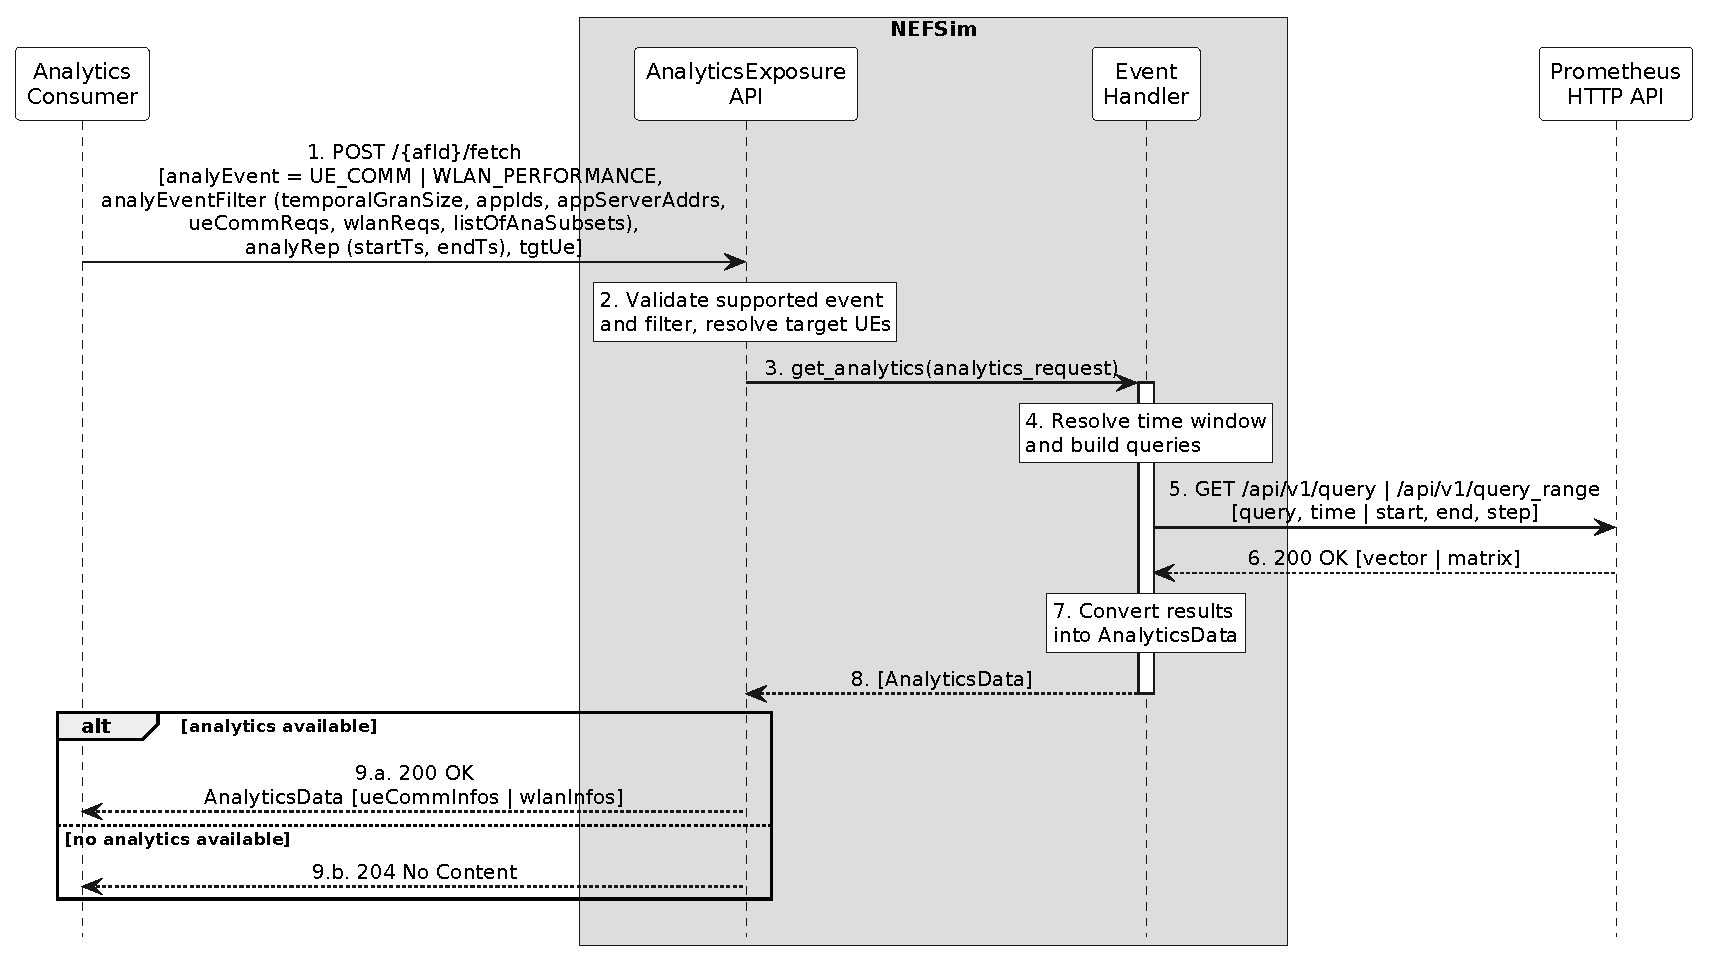
\includegraphics[width=1\linewidth]{figs/plantuml/analytics-exposure-sequence-fetch.pdf}
    \caption{Sequence Diagram for the synchronous retrieval of analytics via the \textit{AnalyticsExposure} \acs{API}}
    \label{fig:impl:exposure:nef:AnalyticsExposure:sequence:fetch}
\end{figure}

Each fetch request identifies the analytics event, the target \acsp{UE} (\texttt{tgtUe}), an optional event filter and the time window to which the analytics refer (step 1). Upon receiving it, the \acs{NEF} validates the requested event and filter, and resolves the target \acsp{UE} (step 2). Both events rely on mapping \acsp{UE} and applications to the \acs{IP} addresses observed in the monitored traffic. Target \acsp{UE} can be selected individually, through their \acs{GPSI}, collectively, through an external group identifier, or all at once, through the any- \acs{UE} indicator. For the \texttt{UE\_COMM} event, the \acs{API} must also identify the applications with which the \acsp{UE} communicate. To this end, a new \acs{NEF}Sim endpoint was introduced to register applications, associating each application identifier with its \acs{IP} and \acs{MAC} addresses. These identifiers can then be referenced in the event filter (\texttt{appIds}), restricting the analytics to the specified applications, or to all registered applications, when omitted. For the \texttt{WLAN\_PERFORMANCE} event, the application server is instead given directly in the event filter (\texttt{appServerAddrs}). The event filter may also specify the subsets of analytics to be reported (\texttt{listOfAnaSubsets}). For the \texttt{WLAN\_PERFORMANCE} event, these determine whether traffic information (\texttt{TRAFFIC\_INFO}) and the number of \acsp{UE} (\texttt{NUMBER\_OF\_UES}) are to be reported, with the remaining subsets being unsupported. The \acs{WLAN} requirements (\texttt{wlanReqs}) additionally restrict the \texttt{WLAN\_PERFORMANCE} analytics to the given (simulated) \acsp{SSID}. Both events also accept ordering criteria (specified in \texttt{ueCommReqs} and \texttt{wlanReqs}), which are applied to the reported entries.

The request is then delegated to the handler of the requested event (step 3). Before building the queries, the handler determines the time window to which the analytics refer (step 4). In synchronous requests, this window is specified through start and/or end timestamps (\texttt{startTs} and \texttt{endTs}), awalys referring to past observations, as the testbed provides no predictive model for future network conditions (e.g. an \acs{NWDAF}). According to \acs{3GPP}~\cite{ETSI_TS_129_520_V18_6_0}, temporal granularity (\texttt{temporalGranSize}) is supported for the \texttt{WLAN\_\allowbreak PERFORMANCE} event, but not for the \texttt{UE\_\allowbreak COMM} event. Hence, for this event the window is further divided into time slots according to the requested \texttt{temporalGranSize}, falling back to a configurable default. This results in a Prometheus range query with a step equal to the slot duration, each sample reporting the throughput and volume observed during the corresponding slot. In contrast, the \texttt{UE\_COMM} event is always evaluated through a single instant query covering the entire window (step 5).

The Prometheus query catalog operates over the byte counters exported by the passive monitoring component, filtered by source and destination \acs{IP} address. Uplink traffic corresponds to packets sent from the \acs{UE} towards the application, and downlink traffic in the opposite direction. Traffic volumes are computed as the increase of the counters over a given interval, and throughput as their per-second rate, converted to bits per second. All queries required by an event are combined into a single Prometheus request, with each sub-query tagged by a distinct label, reducing the number of requests and ensuring the returned samples share the same timestamps. Prometheus answers with an instant vector or a range matrix, respectively (step 6). Moreover, as Prometheus omits time series without samples in the queried window, the handlers explicitly report zeroed values in such cases, so that the absence of traffic is reported as such, rather than as missing analytics.

At the end, the handler converts the query results into the analytics data model of the requested event, i.e. the \texttt{ueCommInfos} or \texttt{wlanInfos} attributes of the \texttt{AnalyticsData} schema (steps 7 and 8), which is returned to the consumer (step 9.a). If no analytics data can be produced for the request, the \acs{NEF} instead responds with no content (step 9.b).

\plan{
    \begin{enumerate}
        \item Come back to the table (CLOSE THE TABLE)
    \end{enumerate}
}